Ben Trout

2014-10-17

Cut pieces for Field, Design and prototype slingshot

\begin{tabular}{|p{5cm}|p{5cm}|}
\hline
Cut pieces for field&
The FRC team I am apart of allowed us to use their wood shop so we could cut the pieces for our field. The first Sunday it was just me and I outlined all the pieces on the two plywood sheets and got started on cutting some of the pieces. I spent a total of three hours the first Sunday with the help of the FRC coaches guiding me, and helping me with the cuts. The second Sunday David and Filip joined me to help cut the rest of the parts. We outlined the rest of the parts on the remaining plywood we had and with the help and guidence of the FRC coach got all our pieces cut. I brought all the pieces to Liberty and now all we have to do is assemble the field elements.
\\
\hline
Design and prototype slingshot&
We started to design the slingshot and have a good idea of what it will look like. With the help of Filip and Alex we designed a piece to hold the ball on Creo. My FRC team will help me print the ball holder with the 3D printer they own. Our method of launching the ball is to have a bar connected to our ball holder, and the other end connected to a wheel. The wheel is connected to a motor. As the wheel spins the printed piece will move up and down. As the piece is pulled down the surgical tubing will get pulled down and as the wheel goes around the ball holder will fling up with the surgical tubing flinging the ball into the air.
\\
\hline
\end{tabular}

\section*{Field Cutting}

The Field assembly went great. I had some adults who know a lot about wood works help me. The planning and cutting went perfect. We didn't mess up on any pieces and now have all the pieces cut. Now that's all left to do is assemble the field which is up to the other teams with me as there guide. 

\section*{Designing and Prototyping slingshot}

The plan for the sling shot has a lot of potential. We got our surgical tubing and tested different lengths and tightness to see what will launch the ball the required distance. We found though that our testing wasn't very usefull, and wouldn't be until we got our actual ball holder. The holders we were using had the surgical tubing attatched in a different method rather than it would. The actual holder would also be a different mass than our current holder we threw together. We desided to stop our testing on the surgical tubing and launching the balls and instead focus on designing the ball holder on Creo. Next week we'll start designing the holder on creo. 

\begin{center}
 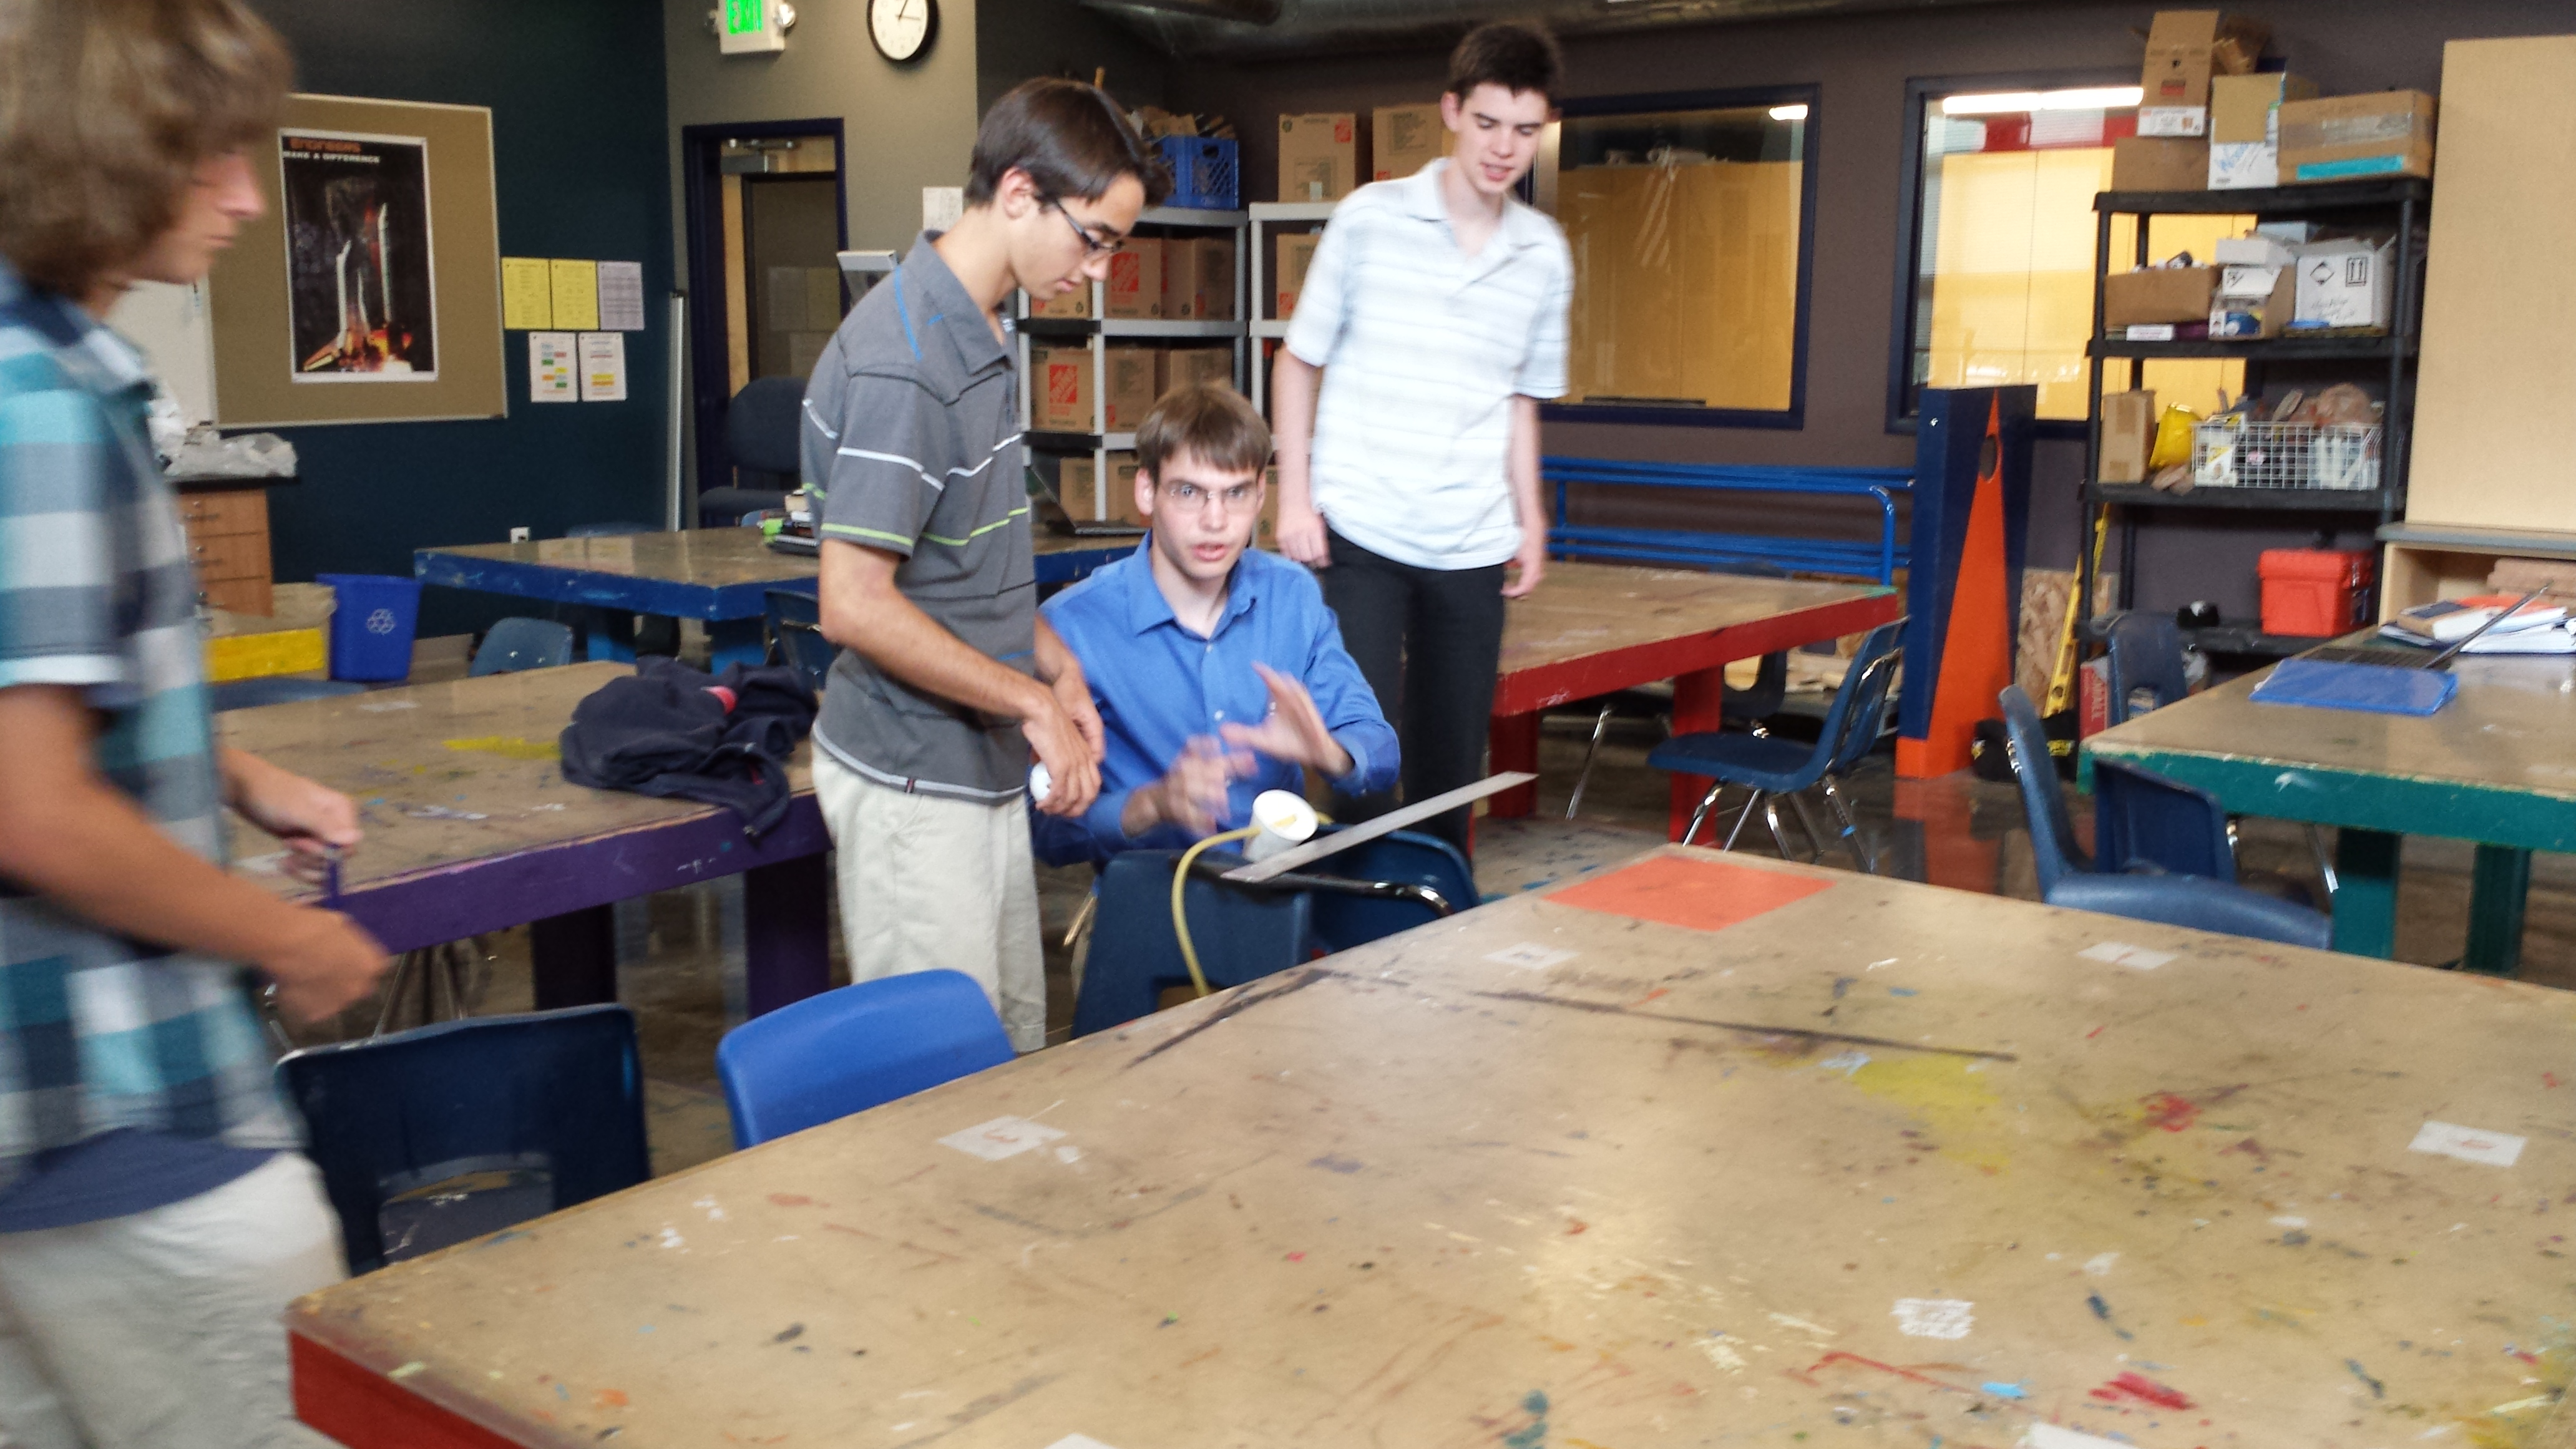
\includegraphics[width=10cm]{./Entries/Images/SlingShotTesting.jpg}
 \end{center}

Our team testing the sling shot

\begin{center}
 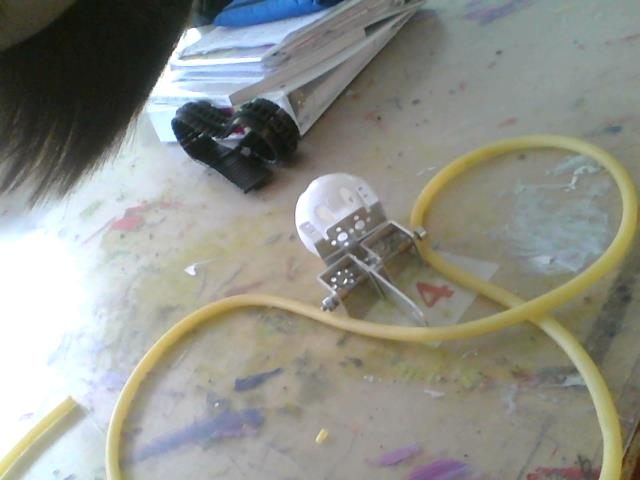
\includegraphics[width=10cm]{./Entries/Images/BallHolder.jpg}
 \end{center}

The original makeshift ball holder that we made out of TETRIX parts


